\documentclass[10pt,letterpaper]{article}
\usepackage[margin=0.9in]{geometry}
\usepackage{times}
\usepackage[T1]{fontenc}
\usepackage{amsmath,amssymb}
\usepackage{booktabs,graphicx,xcolor,caption,enumitem,float}
\usepackage{url}
\usepackage[hidelinks]{hyperref}
\captionsetup{font=small,labelfont=bf}
\setlist{itemsep=1pt,topsep=3pt}
\newcommand{\file}[1]{\path{#1}}
\newcommand{\E}{\mathbb{E}}
\graphicspath{{../figures/}}

\title{Technical Appendix\\[2pt]\large The Missing Band Is a Distribution: Do Generative Bandwidth-Extension Models Sample It?}
\author{Anonymous submission}
\date{}

\begin{document}
\maketitle

\noindent This appendix accompanies the two-page paper. It gives the protocol, the model and training,
exact metric definitions, the derivations behind the argument, the audit of the released models, every metric
for every model on every test set, and the limitations. All numbers are generated from
\file{results/results.json} by \file{results/make_tables.py}; none are typed by hand. The code that produced
them is in \file{code/}, and listening examples are in \file{audio/}.

\tableofcontents

%------------------------------------------------------------------------------------------------------------
\section{What each claim rests on}

\begin{table}[H]
\small\centering
\begin{tabular}{p{0.34\linewidth}p{0.33\linewidth}p{0.25\linewidth}}
\toprule
Claim in the paper & Evidence & Where \\
\midrule
The scoring harness reproduces the released models' published numbers & LSD/ViSQOL of FLowHigh and AP-BWE within 0.011 and 0.02 of their papers & Tab.~\ref{tab:fidelity} \\
With a correct low band the squared error is $E(1+p-2c)$; an empty band maximises SNR when $c\approx0$ & Derivation; measured ceiling; NU-Wave~2's published SNR bounds its level & \S\ref{sec:ceiling}, Tab.~\ref{tab:ceiling}, Fig.~\ref{fig:ceiling} \\
No model recovers the high-band waveform & Coherent fraction $c<0.02$ for every model, 240 utterances & Tab.~\ref{tab:snr} \\
When $c\approx0$, the SNR gap of independent draws is a function of level & Derivation; measured gap against the independent value & \S\ref{sec:avg}, Tab.~\ref{tab:leveldisp} \\
FLowHigh is a regressor: one Euler step returns the conditional mean & Code path, derivation, gap 0.08 against 1.77, rank tails 41\% / 46\% & \S\ref{sec:flowhigh-deriv}, \S\ref{sec:flowhigh}, Fig.~\ref{fig:pit} \\
NU-Wave~2 samples but is too quiet & Gap 0.57 against 0.63; deficit by frame loudness & Tab.~\ref{tab:leveldisp}, Tab.~\ref{tab:levels-wide} \\
AudioSR is biased by band and under-diverse for its level & Per-band levels; gap 2.62 against 3.92; rank tails & Fig.~\ref{fig:levels}, Fig.~\ref{fig:pit} \\
Every model pulls each utterance's level toward the corpus mean & Slope of deficit against the truth's high-band share & Tab.~\ref{tab:slope} \\
The deficit is set mostly by the loss domain, and closed by an energy score & Eight paired arms of one network & Tab.~\ref{tab:t1}, Tab.~\ref{tab:levels-wide} \\
\bottomrule
\end{tabular}
\end{table}

%------------------------------------------------------------------------------------------------------------
\section{Data and protocol}\label{sec:data}

\paragraph{Corpus.} CSTR VCTK 0.92, microphone 1, resampled to 48\,kHz with \texttt{scipy.signal.resample\_poly},
peak-normalised to 0.95. Our training set contains every \texttt{p}-speaker with id $<350$ except p236--p238:
39{,}639 utterances, 37.3\,h. The low-rate input for training is \texttt{resample\_poly} decimation by 4
(48$\to$12\,kHz). Speakers with id $\ge 350$ (LISA's validation split) and \texttt{s5} are excluded from our
training, so every speaker of the released models' test split is unseen by our arms.

\paragraph{Test sets.} All three use the evaluation input of FLowHigh and NU-Wave~2: an order-8 Chebyshev~I
low-pass (0.05\,dB ripple, cut-off 6\,kHz) applied forward-backward (\texttt{sosfiltfilt}), then
\texttt{resample\_poly} to 12\,kHz. The input is written as 32-bit float, so no model sees quantisation the
others do not. Truth is trimmed to a multiple of 3840 samples, so every model's hop divides it.

\begin{table}[H]\small\centering
\begin{tabular}{lllrrl}
\toprule
set & speakers & selection & utterances & seconds & draws per utterance \\
\midrule
\texttt{wide} & p360--p364, p374, p376, s5 & 30 per speaker, evenly spaced & 240 & 731 & 1 \\
\texttt{core} & same & 4 per speaker, evenly spaced & 32 & 88 & 8 \\
\texttt{ourtest} & p236, p237, p238 & 10--11 per speaker & 30 & 165 & 16 (ours), 1 (released) \\
\bottomrule
\end{tabular}
\caption{Test sets. Levels, LSD, SNR and perceptual scores are reported on \texttt{wide}; every probabilistic
metric on \texttt{core}.}
\end{table}

\paragraph{Gain convention.} Each output is scaled so that its energy below 5.5\,kHz matches the truth's.
A model that copies the low band exactly gets gain 1, and its high band is then judged at the level the model
placed it relative to its own low band.

\paragraph{Who saw which speakers.} Table~\ref{tab:seen}. The \texttt{ourtest} speakers are held out from our
training but are in the training sets of FLowHigh, NU-Wave~2 and AP-BWE, so \texttt{ourtest} comparisons with
those models are not fair to our arms. AudioSR's training data includes VCTK with no stated speaker split, so
it may have seen every test speaker.

\begin{table}[H]\small\centering
\begin{tabular}{lccc}
\toprule
model & \texttt{wide}/\texttt{core} speakers & \texttt{ourtest} speakers & source \\
\midrule
ours (all eight arms) & unseen & unseen & our split \\
FLowHigh, NU-Wave 2, AP-BWE & unseen & \textbf{seen} & NU-Wave 2 split (100 training speakers) \\
AudioSR (speech) & possibly seen & possibly seen & multi-domain data including VCTK \\
\bottomrule
\end{tabular}
\caption{Training-set overlap with the test speakers.}\label{tab:seen}
\end{table}

%------------------------------------------------------------------------------------------------------------
\section{Model and training}\label{sec:model}

\paragraph{Network.} LISA: a 1-D convolutional encoder (channels 16, 32, 64, 32; kernels 7, 3, 3, 1; ReLU)
turns the 12\,kHz waveform into one latent per input sample. A 5-layer ReLU MLP of width 144 then decodes the
amplitude at a continuous time coordinate from $[t,z_{i-1},z_i,z_{i+1}]$.
\begin{itemize}
\item \textbf{\texttt{LISAS}} concatenates 8 i.i.d.\ $\mathcal N(0,1)$ channels to the encoder input, at the
input rate: 87{,}777 parameters.
\item \textbf{\texttt{LISASD}} also appends 4 $\mathcal N(0,1)$ channels per 48\,kHz output sample to the decoder
input: 88{,}353 parameters. This follows DISCO Nets and EnScale in putting noise deeper in the network.
\end{itemize}
A draw is one forward pass with fresh noise; at noise temperature $\tau=0$ the network is deterministic. The
deterministic arms use the same class and are trained with the noise held at zero.

\paragraph{Objective.} With $y$ the target and $y_1,y_2$ two draws for the same input, every stochastic arm
minimises the two-draw energy score
\begin{equation}
\mathcal L = \tfrac12\big[d(y,y_1)+d(y,y_2)\big]-\tfrac12\, d(y_1,y_2),\qquad
d = d_{\mathrm{wave}} + \lambda\, d_{\mathrm{spec}} .
\end{equation}
\begin{itemize}
\item $d_{\mathrm{wave}}(a,b)$ is the mean absolute difference of the waveforms.
\item $d_{\mathrm{spec}}$ averages over three Hann STFTs, $(n_{\mathrm{fft}},\mathrm{hop})\in\{(2048,512),
(1024,256),(512,128)\}$.
\item On each STFT it takes the mean of $|\log(|A|+10^{-7})-\log(|B|+10^{-7})|$ (\texttt{es\_marg},
\texttt{es\_dec}).
\item In the ERB arms (\texttt{es\_erb}, \texttt{es\_dec\_erb}), it takes half of that plus half the same L1
on 32 ERB-band log energies, $\tfrac12\log(W|S|^2+10^{-8})$, where $W$ is a 32-band ERB filterbank from 50\,Hz.
\end{itemize}
The deterministic arms minimise $d(y,\hat y)$; \texttt{det\_paper} is LISA's released configuration (L1,
$\lambda=0$). The estimator is unbiased (\S\ref{sec:es}).

\paragraph{Arms.} Table~\ref{tab:t1}. All eight share one batch stream: the sampler is seeded by a fixed label,
so every arm sees identical segments in identical order, and differences between arms are paired.

\paragraph{Optimisation.}
\begin{itemize}
\item Adam, learning rate $10^{-3}$, halved at 20, 40, 50, 60, 70 and 80\% of training (LISA's schedule scaled
to our step count), so the final rate is $\mathrm{lr}_0/64$.
\item Gradient-norm clipping at $10^{-3}$, per arm.
\item Batch 64 one-second segments; 104{,}950 steps, which is 50 epochs of the 37.3\,h corpus.
\item bf16 autocast on the network, all distances and STFTs in fp32, TF32, fused Adam. The decoder's anchor
jitter is kept from LISA.
\item One arm per NVIDIA RTX PRO 6000 (Blackwell) GPU: 105\,ms per step, about 3.1\,h per arm.
\item One training seed per arm.
\end{itemize}
Training curves are in Fig.~\ref{fig:train}; full histories and logs are in \file{results/training/}.

%------------------------------------------------------------------------------------------------------------
\section{Metric definitions}\label{sec:metrics}

All metrics come from one scorer, \file{code/sota/score.py}, applied to every model's saved outputs. The high
band (HB) is 6--24\,kHz. Per-draw quantities are averaged over draws, then over utterances.
\begin{description}[leftmargin=1.2em,style=nextline]
\item[Deficit] The evaluation STFT is Hann, 1024/256. Take third-octave bands from 6\,kHz to 24\,kHz
(centres 6.7, 8.5, 10.7, 13.4, 16.9 and 21.3\,kHz). In each band compute $10\log_{10}(E_{\mathrm{out}}/E_{\mathrm{true}})$
over all frames, then average over bands. 0 is right; negative is too quiet.
\begin{itemize}
\item \emph{deficit bb} is the energy-weighted ratio over the whole band.
\item \emph{loud / mid / quiet} restrict to the truth's frames in the top 25\%, middle 50\% and bottom 25\% of
frame magnitude.
\end{itemize}
\item[LSD] Hann 2048/512, $\log_{10}|X|^2$, RMS over frequency, mean over frames. This is the basis of NU-Wave~2's
\texttt{for\_test.py}. LSD-HF and LSD-LF split at 6\,kHz.
\item[SNR] $10\log_{10}(\|y\|^2/\|y-\hat y\|^2)$ per whole utterance, averaged in dB over utterances.
\begin{itemize}
\item \emph{Ceiling}: the truth with its HB removed (a brick wall at 6\,kHz).
\item \emph{vs ceiling}: the model's SNR minus that ceiling.
\end{itemize}
\item[Coherent fraction, $\kappa$] Computed per HB third-octave band on the STFT, then averaged over bands:
$c=\mathrm{Re}\langle Y,W\rangle/\langle Y,Y\rangle$ (the predictable fraction) and
$\kappa=\mathrm{Re}\langle Y,W\rangle/\langle W,W\rangle$ (1 = informative energy, 0 = energy unrelated to the truth).
\item[CRPS] The features are HB log-magnitudes $\log(|X|+10^{-8})$ (natural log; one unit is 8.69\,dB) on the
1024/256 STFT, bins $k\ge128$. For each bin, with $M$ draws $x_1,\dots,x_M$ and truth $y$:
\[
\mathrm{CRPS}_{\mathrm{fair}}=\frac1M\sum_j|x_j-y|-\frac{1}{2M(M-1)}\sum_{j\neq k}|x_j-x_k| .
\]
This is averaged over bins, frames and utterances. The tables' ``CRPS'' column for an ensemble is this fair
estimator. The appendix also reports the all-pairs estimator, which divides by $M^2$; its expected value
exceeds the infinite-ensemble CRPS by $\E|X-X'|/(2M)$ \cite{ferro2008}. A one-output model scores its mean
absolute error, which is the CRPS of a point forecast.
\item[Sliced CRPS] The all-pairs CRPS on 32 fixed random unit projections of each frame's HB log-magnitude
vector. It is sensitive to dependence across bins.
\item[PIT tails] The rank of the truth among the $M$ draws in each HB bin, pooled over bins and utterances.
\emph{PIT low} and \emph{PIT high} are the shares where the truth is below all draws and above all draws. For a
calibrated ensemble each is $1/(M+1)=0.111$ at $M=8$.
\item[Spread] The pooled ratio $\sum_u s_u^2(1+1/M)\big/\sum_u\|y_u-\bar x_u\|^2$, computed on the HB waveform,
where $s_u^2$ is the unbiased ensemble variance and $\bar x_u$ the ensemble mean. It is 1 for a calibrated
ensemble and below 1 when the ensemble is under-dispersed.
\item[Gap] $10\log_{10}\big(\mathrm{mean}_i\|y-x_i\|^2/\|y-\bar x\|^2\big)$ on the HB waveform. For a
calibrated ensemble it is $10\log_{10}(2/(1+1/M))=2.50$\,dB at $M=8$ (\S\ref{sec:avg}).
\item[corr err] $\|C_{\mathrm{true}}-C_{\mathrm{draw}}\|_F$, where $C$ is the correlation matrix of 16 HB
frequency groups of log-magnitude, pooled over frames and utterances.
\item[Slope] The least-squares slope of the per-utterance deficit (dB) against the truth's HB energy share (dB),
on \texttt{wide} ($n=240$). A slope of 0 means the model tracks each utterance's brightness; $-1$ means it
emits a fixed level.
\item[Perceptual] ViSQOL v3 in audio mode at 48\,kHz (and NSIM), and in speech mode at 16\,kHz; wide-band PESQ.
All on draw 0.
\end{description}

%------------------------------------------------------------------------------------------------------------
\section{Derivations}\label{sec:deriv}

\subsection{The high-band error and the SNR ceiling}\label{sec:ceiling}
Let the truth's HB have energy $E$, the output's HB energy $pE$, and $c=\mathrm{Re}\langle Y_H,W_H\rangle/E$.
With a perfect low band,
\begin{equation}
\|y-\hat y\|^2=\|Y_H-W_H\|^2=E+pE-2cE=E(1+p-2c).
\end{equation}
An empty band ($p=c=0$) costs exactly $E$, so its SNR is the ceiling $C\approx-10\log_{10}(\text{HB share})$.
A model beats $C$ only if $c>p/2$. An incoherent band at the right level ($p=1$, $c\approx0$) costs
$10\log_{10}2=3.0$\,dB. This matches the measured $-2.8$\,dB of FLowHigh, $-3.1$\,dB of AP-BWE and $-2.8$\,dB of
our sampler against the ceiling on \texttt{wide} (Tab.~\ref{tab:snr}).

Conversely, a reported SNR $S$ bounds the HB level: $p\le10^{(C-S)/10}-1$, since any low-band error only
lowers $S$; with nonzero coherence the bound is $p\le10^{(C-S)/10}-1+2c$. As a consistency check, take
NU-Wave~2's own Table~1, where the ``Input'' row is its ceiling: at 12\,kHz, $C-S=0.5$\,dB, and with its
measured $c=0.009$ this gives $p\le0.14$, i.e.\ at most $-8.5$\,dB. We measure a broadband deficit of
$-8.9$\,dB. The identity reads a published SNR as a statement about high-band level, and our harness agrees
with NU-Wave~2's own number.
The ceiling measured on our 240 utterances is in Table~\ref{tab:ceiling}, and reported SNRs against it in
Fig.~\ref{fig:ceiling}.

\subsection{Averaging draws, and the calibration target}\label{sec:avg}
For draws $x_1,\dots,x_M$ with HB components that are mutually incoherent and of equal energy,
$\E\|\bar x_H\|^2=\E\|x_H\|^2/M$: the waveform mean loses $10\log_{10}M$\,dB. A regressor trained on
squared error estimates the $M\to\infty$ mean, which is the argument for why point training yields a quiet band.

If $y$ and the $x_i$ are exchangeable given the input (a calibrated sampler),
$\E\|y-x_i\|^2=2\sigma^2$ and $\E\|y-\bar x\|^2=\sigma^2(1+1/M)$. This gives the gap target
$10\log_{10}(2/(1+1/M))$ and the spread normalisation above.

The log-domain mean behaves differently. If a bin's power is exponentially distributed, as for a circular
Gaussian bin, then $\E\log P=\log\E P-\gamma$. The per-bin mean of log-magnitudes therefore sits
$10\gamma/\ln10=2.51$\,dB below the draws' energy as $M\to\infty$, where $\gamma$ is the Euler--Mascheroni
constant.

\paragraph{Scorer check on synthetic data.} Build a set whose HB draws are fresh noise of the true envelope and
level, so the truth is exchangeable with the draws by construction.
\begin{itemize}
\item \file{score.py} returns gap 2.50\,dB (target 2.50), spread 0.999 (target 1), and PIT tails 0.109 and 0.125
(target 0.111).
\item \file{mean_of_M.py} returns waveform-mean deficits of $-3.01$, $-6.02$ and $-9.03$\,dB at $M=2,4,8$
(predicted $-3.01$, $-6.02$, $-9.03$), and a log-mean deficit of $-2.63$\,dB at $M=8$ (limit $-2.51$).
\end{itemize}
\file{code/sota/mean_of_M.py} computes the mean-of-$M$ table on real draws, and \file{code/sota/run_all.sh}
runs it.

\subsection{The two-draw energy score: unbiased and proper}\label{sec:es}
For any $d$, $\E\big[\tfrac12(d(y,Y_1)+d(y,Y_2))-\tfrac12 d(Y_1,Y_2)\big]=\E d(y,Y)-\tfrac12\E d(Y,Y')$, the
energy score, with no finite-ensemble bias \cite{gneiting2007,gritsenko2020}. Its propriety depends on $d$.

Here $d$ is an $L_1$ sum over waveform samples and over STFT and ERB features. The energy score of a sum of
coordinatewise absolute differences is the sum of per-coordinate CRPS terms. It is therefore proper, and
strictly proper for the marginal distribution of each coordinate, but not for their joint distribution: the
$L_1$ metric on $\mathbb R^n$ is of negative type but not of strong negative type.

The multi-scale STFT and ERB terms add transformed coordinates, which keeps the score proper
\cite{allen2023}, but dependence between bins is constrained only through those transforms. This is why the
sliced CRPS and the band-correlation error are reported next to the per-bin CRPS.

\subsection{CRPS of a point forecast}\label{sec:point}
For a point forecast $m$, CRPS equals $\E|Y-m|$. For any $m$, $\tfrac12\E|Y-Y'|\le\E|Y-m|$, so a calibrated
sampler has lower expected CRPS than every point forecast. The comparison between samplers and deterministic
models on CRPS (Table~\ref{tab:t1}) is therefore expected by construction. The informative comparisons are
among ensembles, and between ensembles and the calibration targets.

\subsection{One Euler step of FLowHigh returns the conditional mean}\label{sec:flowhigh-deriv}
FLowHigh's path (\texttt{independent\_cfm\_adaptive}) trains on $x_t=t\,x_1+(1-t)x_0+\sigma_t\epsilon$ with
$\sigma_t=1-(1-\sigma_{\min})t$ and target $u=(x_1-x_0)-(1-\sigma_{\min})\epsilon$. Here $x_0$ is the input's mel
spectrogram, $x_1$ the target's, and $\sigma_{\min}=10^{-4}$.

In training, the network at $t=0$ sees $x=x_0+\epsilon$ together with $x_0$ (as conditioning), so
$\epsilon=x-x_0$ is identified. The optimal field is therefore
$v^*(x,0)=\E[x_1\mid x_0]-x_0-(1-\sigma_{\min})(x-x_0)$. Starting instead from $x=x_0+s\epsilon$, one Euler step
returns
\begin{equation}
x+v^*(x,0)=\E[x_1\mid x_0]+\sigma_{\min}\,s\,\epsilon ,
\end{equation}
the conditional mean for any start-noise scale $s$, then a deterministic vocoder. This follows from the
rectified-flow identity $v(x,t)=\E[X_1-X_0\mid X_t=x]$ \cite{liu2022}. Restoring the trained prior ($s=1$) cannot
restore the spread at one step (\S\ref{sec:flowhigh}).

%------------------------------------------------------------------------------------------------------------
\section{The released models}\label{sec:released}

Each model runs through its own inference code on the same input (\file{code/sota/run_models.py}), with the
seed set per draw.

\begin{table}[H]\small\centering
\begin{tabular}{p{0.13\linewidth}p{0.3\linewidth}p{0.2\linewidth}p{0.27\linewidth}}
\toprule
model & release used & sampling & notes \\
\midrule
FLowHigh & official code (MIT), \texttt{FLowHigh\_indep\_adaptive\_400k} + BigVGAN 48\,kHz & 1 Euler step (their setting) & deterministic as shipped (\S\ref{sec:flowhigh}) \\
NU-Wave 2 & official code (BSD), official checkpoint & 8 DDIM steps, their schedule & loaded without pytorch-lightning; weights unchanged \\
AP-BWE & official code (MIT), 12$\to$48\,kHz checkpoint & one pass & not level-invariant; fed at the stored level \\
AudioSR & official package, \texttt{speech} checkpoint & 50 DDIM steps, guidance 3.5 (CLI defaults) & its low band also varies between draws \\
\bottomrule
\end{tabular}
\caption{Released models as run. AP-BWE was also scored on its own paper's sinc input (``own sinc input'' rows).}
\end{table}

\begin{table}[H]\small\centering
\begin{tabular}{lrrrrl}
\toprule
model & LSD reported & LSD ours & ViSQOL reported & ViSQOL ours & reported in \\
\midrule
FLowHigh & 0.75 & 0.761 & 3.61 & 3.61 & FLowHigh, Tab. I \\
AP-BWE & 0.78 & 0.780 & 3.46 & 3.48 & AP-BWE, Tab. V \\
NU-Wave 2 & 0.94 & 0.989 & 2.75 & 2.57 & AP-BWE, Tab. V (re-run) \\
\bottomrule
\end{tabular}

\caption{Does the harness reproduce each model's own numbers? \texttt{wide}, 240 utterances. Reported values
are from the papers' 12$\to$48\,kHz VCTK tables (NU-Wave~2's as re-run by AP-BWE; its own paper reports SNR,
21.6\,dB, against our 21.3\,dB).}\label{tab:fidelity}
\end{table}

\subsection{FLowHigh}\label{sec:flowhigh}
The released \texttt{inference.py} calls \texttt{sample(..., std\_2 = 1.)} without \texttt{std\_1}. Inside
\texttt{sample()}, \texttt{if std\_1 is None or std\_2 is None: std\_1 = 1.0; std\_2 = self.sigma}. So the start
point is $x_0+10^{-4}\epsilon$, while training starts from $x_0+\epsilon$ ($\sigma_0=1$). The README recommends
\texttt{--time\_step 1 --sigma 0.0001}. The explicit \texttt{std\_2 = 1.} suggests the override is unintended.
\file{code/patches/flowhigh_inference_restore_prior.diff} is the one-line change that keeps the trained prior.

Measured on \texttt{core}:
\begin{itemize}
\item As shipped, the HB spread ratio is $2\times10^{-9}$.
\item With the prior restored it is $0.023$, and the truth falls below or above all eight draws in 41\% and 46\%
of HB bins (Fig.~\ref{fig:pit}).
\end{itemize}
This is what \S\ref{sec:flowhigh-deriv} predicts: the override is real, but one-step sampling is what forces
the mean. In Table~\ref{tab:t2}, FLowHigh's deficit, LSD and ViSQOL are as shipped, and its spread and CRPS are
from the prior-restored run, the most favourable reading for it.

\subsection{Cost}
\begin{table}[H]\small\centering
\begin{tabular}{lrrll}
\toprule
model & params & RTF & device & sampling \\
\midrule
FLowHigh & 49.4 M & 1.237 & cpu & 1 Euler step (their setting) \\
AP-BWE & 29.8 M & 0.071 & cpu & 1 pass \\
NU-Wave 2 & 1.7 M & 4.985 & cpu & 8 DDIM steps \\
AudioSR (speech) & 672.0 M & 4.611 & mps & 50 DDIM steps \\
\bottomrule
\end{tabular}

\caption{Parameters, and real-time factor (wall seconds per second of audio) on an Apple M4, each model alone,
warm, median of three. Our 88\,k network runs at about 0.017 on the same CPU.}
\end{table}

%------------------------------------------------------------------------------------------------------------
\section{Results}\label{sec:results}

\subsection{Full versions of the paper's tables}
\begin{table}[H]\small\centering
\begin{tabular}{llrlrr}
\toprule
arm & one change & deficit (dB) & step & spread & CRPS \\
\midrule
det\_paper & LISA recipe (L1, $\lambda{=}0$) & $-$21.78 & -- & -- & 2.853 \\
det & + log-magnitude term, $\lambda{=}0.01$ & $-$6.18 & 15.6 [det\_paper] & -- & 0.889 \\
es\_marg & point $\to$ draw (energy score) & $-$1.05 & 5.1 [det] & 0.526 & 0.537 \\
es\_dec & + decoder noise & $-$1.12 & $-$0.1 [es\_marg] & 0.499 & 0.535 \\
es\_erb & + ERB-band term & $-$1.08 & 0.0 [es\_marg] & 0.442 & 0.512 \\
es\_erb, $\lambda{=}0.1$ & $\lambda \times 10$ & $-$0.63 & 0.5 [es\_erb] & 0.479 & 0.515 \\
es\_erb, $\lambda{=}0.001$ & $\lambda / 10$ & $-$5.73 & $-$4.6 [es\_erb] & 0.225 & 0.683 \\
es\_dec\_erb, $\lambda{=}0.1$ & decoder noise + ERB, $\lambda{=}0.1$ & $-$0.70 & -- & 0.464 & 0.514 \\
\bottomrule
\end{tabular}

\caption{All eight arms of one network (the paper's Table~2 shows six). Deficit on \texttt{wide} (240 utterances, one
draw); step = change of deficit against the arm in brackets. Spread and CRPS on \texttt{core} (32 utterances,
8 draws); a deterministic arm's CRPS is its MAE.}\label{tab:t1}
\end{table}

\begin{table}[H]\small\centering
\begin{tabular}{lrrrrrrr}
\toprule
model & params & deficit (dB) & LSD & ViSQOL & spread & CRPS & slope \\
\midrule
FLowHigh & 49.4 M & $-$1.60 & 0.761 & 3.61 & 0.023 & 0.682 & $-$0.07 \\
AP-BWE & 29.8 M & $-$1.38 & 0.780 & 3.48 & -- & 0.777 & $-$0.12 \\
NU-Wave 2 & 1.7 M & $-$7.96 & 0.989 & 2.57 & 0.094 & 0.583 & $-$0.32 \\
AudioSR (speech) & 672.0 M & $-$0.60 & 1.561 & 2.41 & 0.765 & 1.243 & $-$0.34 \\
det & 88 k & $-$6.18 & 0.864 & 3.13 & -- & 0.889 & $-$0.22 \\
es\_dec\_erb, $\lambda{=}0.1$ & 88 k & $-$0.70 & 0.895 & 2.83 & 0.464 & 0.514 & $-$0.23 \\
\bottomrule
\end{tabular}

\caption{Released models against two of our arms (the paper's Table~1, with spread and slope). Deficit, LSD and ViSQOL (audio
mode) are on \texttt{wide}; spread and CRPS on \texttt{core}; slope on \texttt{wide} ($n=240$ for every
model). FLowHigh's spread and CRPS are with its prior restored.}\label{tab:t2}
\end{table}

\subsection{Levels}
\begin{table}[H]\small\centering
\resizebox{\linewidth}{!}{\begin{tabular}{lrrrrrrrr}
\toprule
condition & deficit & deficit bb & loud & mid & quiet & LSD & LSD-HF & LSD-LF \\
\midrule
FLowHigh & $-$1.60 & $-$2.33 & $-$1.71 & $-$1.34 & $-$1.03 & 0.761 & 0.869 & 0.212 \\
FLowHigh, prior restored & $-$2.38 & $-$3.09 & $-$2.45 & $-$2.05 & $-$1.28 & 0.761 & 0.869 & 0.211 \\
AP-BWE & $-$1.38 & $-$1.23 & $-$1.74 & $-$0.90 & 0.18 & 0.780 & 0.894 & 0.179 \\
AP-BWE, own sinc input & $-$1.51 & $-$1.41 & $-$1.84 & $-$1.16 & $-$0.16 & 0.781 & 0.893 & 0.212 \\
NU-Wave 2 & $-$7.96 & $-$8.93 & $-$8.96 & $-$5.17 & 4.72 & 0.989 & 1.117 & 0.351 \\
AudioSR (speech) & $-$0.60 & 2.17 & $-$1.03 & 0.28 & $-$5.20 & 1.561 & 1.778 & 0.470 \\
det\_paper & $-$21.78 & $-$15.66 & $-$20.89 & $-$23.50 & $-$21.30 & 2.319 & 2.674 & 0.210 \\
det & $-$6.18 & $-$7.38 & $-$6.74 & $-$3.87 & $-$2.26 & 0.864 & 0.987 & 0.237 \\
es\_marg & $-$1.05 & $-$1.34 & $-$1.90 & 1.53 & $-$2.20 & 0.929 & 1.036 & 0.432 \\
es\_dec & $-$1.12 & $-$1.45 & $-$2.26 & 1.87 & $-$1.74 & 0.919 & 1.032 & 0.399 \\
es\_erb & $-$1.08 & $-$1.64 & $-$1.86 & 1.60 & $-$1.17 & 0.902 & 1.012 & 0.398 \\
es\_erb, $\lambda{=}0.1$ & $-$0.63 & $-$1.31 & $-$1.63 & 1.98 & $-$1.20 & 0.894 & 1.012 & 0.326 \\
es\_erb, $\lambda{=}0.001$ & $-$5.73 & $-$4.07 & $-$6.25 & $-$3.41 & $-$3.83 & 1.025 & 1.109 & 0.668 \\
es\_dec\_erb, $\lambda{=}0.1$ & $-$0.70 & $-$1.44 & $-$1.53 & 1.87 & $-$1.58 & 0.895 & 1.012 & 0.336 \\
\bottomrule
\end{tabular}
}
\caption{\texttt{wide}: deficits (dB) and LSD for every condition. Loud, mid and quiet are the truth's frames by
loudness. NU-Wave~2's band is $-9.0$\,dB on loud frames and $+4.7$\,dB on quiet ones: it stays on between
words.}\label{tab:levels-wide}
\end{table}

\begin{table}[H]\small\centering
\resizebox{\linewidth}{!}{\begin{tabular}{lrrrrrrrr}
\toprule
condition & deficit & deficit bb & loud & mid & quiet & LSD & LSD-HF & LSD-LF \\
\midrule
FLowHigh & $-$1.18 & $-$1.95 & $-$1.08 & $-$1.41 & $-$0.89 & 0.760 & 0.868 & 0.215 \\
FLowHigh, prior restored & $-$1.86 & $-$2.61 & $-$1.74 & $-$2.05 & $-$1.15 & 0.760 & 0.868 & 0.215 \\
AP-BWE & $-$1.11 & $-$1.07 & $-$1.23 & $-$0.59 & 0.16 & 0.775 & 0.888 & 0.180 \\
AP-BWE, own sinc input & $-$1.20 & $-$1.24 & $-$1.27 & $-$0.87 & $-$0.17 & 0.776 & 0.887 & 0.212 \\
NU-Wave 2 & $-$7.85 & $-$8.73 & $-$8.61 & $-$5.46 & 4.24 & 0.982 & 1.109 & 0.346 \\
AudioSR (speech) & $-$0.99 & 2.24 & $-$1.20 & $-$0.07 & $-$4.87 & 1.552 & 1.761 & 0.519 \\
det\_paper & $-$21.31 & $-$15.23 & $-$20.48 & $-$23.17 & $-$22.06 & 2.350 & 2.709 & 0.208 \\
det & $-$5.82 & $-$7.04 & $-$6.28 & $-$3.63 & $-$2.37 & 0.863 & 0.985 & 0.236 \\
es\_marg & $-$0.72 & $-$1.08 & $-$1.53 & 1.88 & $-$1.88 & 0.924 & 1.032 & 0.429 \\
es\_dec & $-$0.98 & $-$1.34 & $-$1.93 & 1.86 & $-$1.68 & 0.914 & 1.027 & 0.396 \\
es\_erb & $-$1.08 & $-$1.70 & $-$1.80 & 1.68 & $-$1.32 & 0.895 & 1.005 & 0.393 \\
es\_erb, $\lambda{=}0.1$ & $-$0.31 & $-$1.07 & $-$1.17 & 2.07 & $-$1.35 & 0.891 & 1.009 & 0.324 \\
es\_erb, $\lambda{=}0.001$ & $-$5.67 & $-$4.13 & $-$6.13 & $-$3.44 & $-$4.37 & 1.029 & 1.112 & 0.672 \\
es\_dec\_erb, $\lambda{=}0.1$ & $-$0.29 & $-$1.10 & $-$1.02 & 2.03 & $-$1.73 & 0.891 & 1.007 & 0.335 \\
\bottomrule
\end{tabular}
}
\caption{\texttt{core}, the utterances on which calibration is measured.}
\end{table}

\begin{table}[H]\small\centering
\resizebox{0.9\linewidth}{!}{\begin{tabular}{lrrrrrrrr}
\toprule
condition & deficit & deficit bb & loud & mid & quiet & LSD & LSD-HF & LSD-LF \\
\midrule
FLowHigh & $-$1.00 & $-$1.00 & $-$1.11 & $-$0.26 & 0.40 & 0.740 & 0.844 & 0.224 \\
AP-BWE & $-$3.12 & $-$2.95 & $-$3.26 & $-$2.35 & 0.06 & 0.779 & 0.893 & 0.182 \\
det\_paper & $-$25.16 & $-$20.88 & $-$25.05 & $-$24.34 & $-$18.63 & 2.167 & 2.498 & 0.206 \\
det & $-$10.16 & $-$11.56 & $-$11.17 & $-$6.76 & $-$0.75 & 0.885 & 1.012 & 0.237 \\
es\_marg & $-$4.53 & $-$5.05 & $-$5.90 & $-$0.79 & $-$0.23 & 0.958 & 1.066 & 0.443 \\
es\_dec & $-$4.77 & $-$5.31 & $-$6.34 & $-$0.77 & 0.19 & 0.937 & 1.049 & 0.410 \\
es\_erb & $-$4.73 & $-$5.43 & $-$6.01 & $-$0.92 & 0.82 & 0.926 & 1.038 & 0.405 \\
es\_erb, $\lambda{=}0.1$ & $-$4.13 & $-$4.97 & $-$5.53 & $-$0.41 & 0.63 & 0.914 & 1.034 & 0.331 \\
es\_erb, $\lambda{=}0.001$ & $-$8.87 & $-$7.49 & $-$9.90 & $-$5.44 & $-$1.18 & 1.029 & 1.118 & 0.629 \\
es\_dec\_erb, $\lambda{=}0.1$ & $-$4.26 & $-$5.19 & $-$5.66 & $-$0.51 & 0.34 & 0.914 & 1.033 & 0.340 \\
\bottomrule
\end{tabular}
}
\caption{\texttt{ourtest} (p236--p238). These speakers are in the training sets of FLowHigh and AP-BWE
(Table~\ref{tab:seen}).}
\end{table}

\begin{figure}[H]\centering
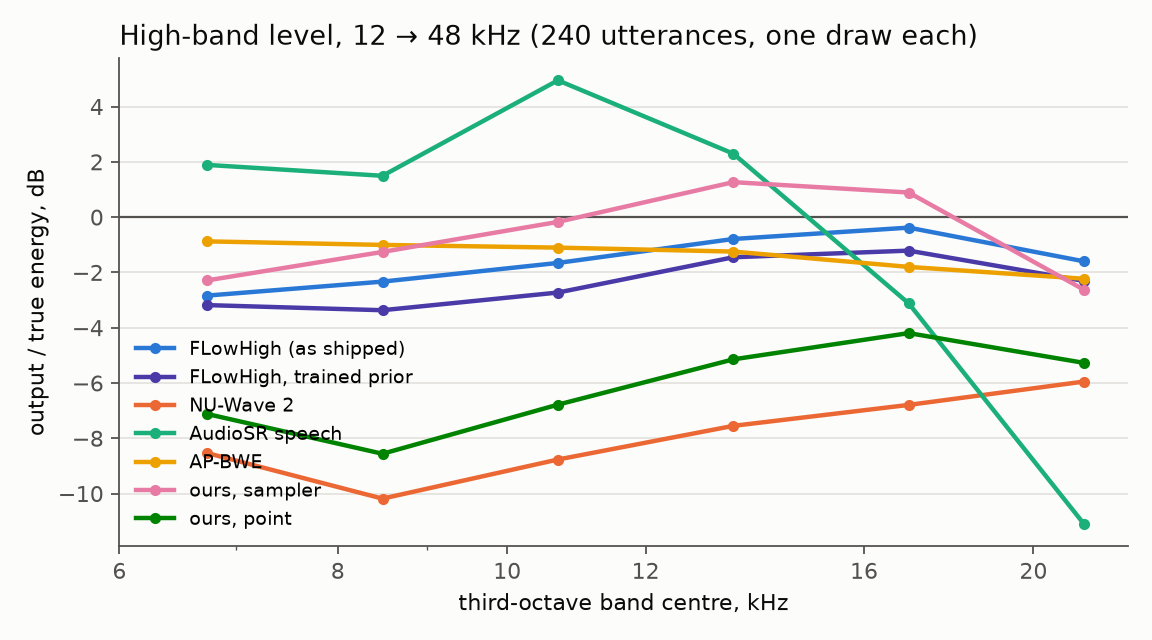
\includegraphics[width=0.8\linewidth]{sota_levels.png}
\caption{High-band level per third-octave band on \texttt{wide}. AudioSR's small mean deficit hides $+5$\,dB at
11\,kHz and $-11$\,dB at 21\,kHz.}\label{fig:levels}
\end{figure}

\subsection{SNR, the ceiling, and coherence}
\begin{table}[H]\small\centering
\begin{tabular}{lr}
\toprule
input rate & empty-band SNR ceiling (dB) \\
\midrule
8 kHz & 19.00 \\
12 kHz & 22.02 \\
16 kHz & 24.67 \\
24 kHz & 30.00 \\
\bottomrule
\end{tabular}

\caption{Empty-band SNR ceiling on \texttt{wide} (true low band, nothing above the input's Nyquist frequency),
per input rate.}\label{tab:ceiling}
\end{table}

\begin{table}[H]\small\centering
\begin{tabular}{lrrrr}
\toprule
condition & SNR (dB) & vs ceiling & coherent frac. & $\kappa$ \\
\midrule
FLowHigh & 19.18 & $-$2.84 & 0.0014 & 0.002 \\
FLowHigh, prior restored & 19.45 & $-$2.57 & 0.0015 & 0.003 \\
AP-BWE & 18.95 & $-$3.07 & 0.0164 & 0.020 \\
AP-BWE, own sinc input & 19.05 & $-$2.96 & 0.0217 & 0.027 \\
NU-Wave 2 & 21.26 & $-$0.76 & 0.0094 & 0.065 \\
AudioSR (speech) & 15.44 & $-$6.58 & $-$0.0005 & 0.000 \\
det\_paper & 21.87 & $-$0.15 & 0.0105 & 0.145 \\
det & 21.19 & $-$0.83 & 0.0143 & 0.071 \\
es\_marg & 18.83 & $-$3.18 & 0.0126 & 0.014 \\
es\_dec & 18.89 & $-$3.13 & 0.0125 & 0.015 \\
es\_erb & 18.96 & $-$3.06 & 0.0094 & 0.016 \\
es\_erb, $\lambda{=}0.1$ & 19.17 & $-$2.85 & 0.0145 & 0.022 \\
es\_erb, $\lambda{=}0.001$ & 18.59 & $-$3.43 & 0.0125 & 0.021 \\
es\_dec\_erb, $\lambda{=}0.1$ & 19.26 & $-$2.76 & 0.0151 & 0.025 \\
\bottomrule
\end{tabular}

\caption{\texttt{wide}. Every model sits below the ceiling. The coherent fraction is below 0.02 for every model
on the Chebyshev input; AP-BWE on its own sinc input reaches 0.022.}\label{tab:snr}
\end{table}

\begin{figure}[H]\centering
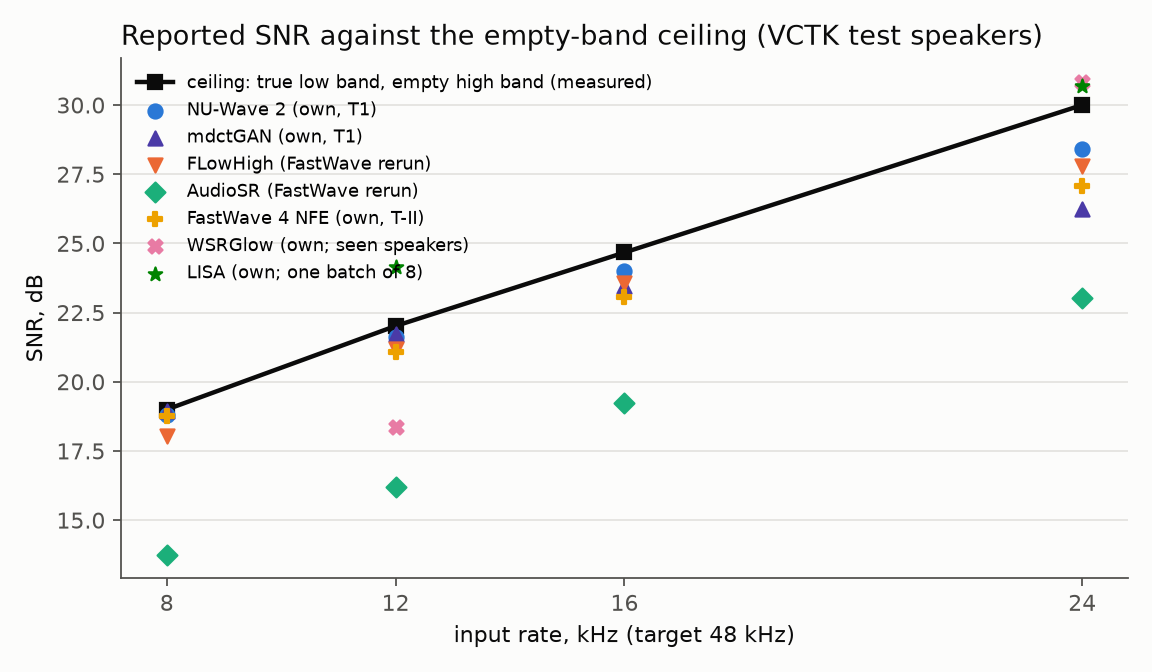
\includegraphics[width=0.75\linewidth]{sota_ceiling.png}
\caption{Reported SNRs from the literature against the ceiling measured on the same test speakers. Markers
above the line come from protocols that differ from the ceiling's, as labelled (speakers seen in training, or
one batch of eight clips).}\label{fig:ceiling}
\end{figure}

\subsection{Calibration and proper scores}
\begin{table}[H]\small\centering
\resizebox{\linewidth}{!}{\begin{tabular}{lrrrrrrrr}
\toprule
condition & gap HB (dB) & spread & PIT low & PIT high & CRPS & CRPS fair & sliced & corr err \\
\midrule
FLowHigh & 0.00 & 0.000 & 0.487 & 0.513 & 0.756 & 0.756 & 0.784 & 0.478 \\
FLowHigh, prior restored & 0.08 & 0.023 & 0.408 & 0.460 & 0.692 & 0.682 & 0.705 & 0.500 \\
NU-Wave 2 & 0.57 & 0.094 & 0.132 & 0.217 & 0.638 & 0.583 & 0.614 & 0.863 \\
AudioSR (speech) & 2.62 & 0.765 & 0.110 & 0.520 & 1.287 & 1.243 & 1.204 & 0.782 \\
es\_marg & 2.21 & 0.526 & 0.098 & 0.241 & 0.591 & 0.537 & 0.576 & 0.374 \\
es\_dec & 2.13 & 0.499 & 0.098 & 0.237 & 0.589 & 0.535 & 0.572 & 0.383 \\
es\_erb & 2.03 & 0.442 & 0.111 & 0.211 & 0.564 & 0.512 & 0.555 & 0.289 \\
es\_erb, $\lambda{=}0.1$ & 2.07 & 0.479 & 0.108 & 0.213 & 0.569 & 0.515 & 0.559 & 0.415 \\
es\_erb, $\lambda{=}0.001$ & 1.16 & 0.225 & 0.097 & 0.421 & 0.726 & 0.683 & 0.677 & 0.476 \\
es\_dec\_erb, $\lambda{=}0.1$ & 2.07 & 0.464 & 0.107 & 0.212 & 0.567 & 0.514 & 0.560 & 0.438 \\
\bottomrule
\end{tabular}
}
\caption{\texttt{core}, $M=8$. Ideals: gap 2.50\,dB, spread 1, PIT low = PIT high = 0.111, corr err 0.
``CRPS'' is the all-pairs estimator; ``CRPS fair'' is the one used in the paper.}\label{tab:calib}
\end{table}

\noindent The two waveform-domain measures do not always agree. Our sampler's gap (2.07\,dB) is within 17\% of
the calibrated 2.50\,dB, while its pooled spread ratio (0.46) says it is under-dispersed. Both are dominated
by output level when the band is incoherent with the truth (\S\ref{sec:ceiling}), so neither is read here as
a pure measure of diversity.

\begin{table}[H]\small\centering
\resizebox{\linewidth}{!}{\begin{tabular}{lrrrrrrr}
\toprule
condition & HB level (dB) & gap & gap if indep. & spread & spread if indep. & PIT low & PIT high \\
\midrule
FLowHigh & $-$1.9 & 0.00 & 1.99 & 0.000 & 0.618 & 0.487 & 0.513 \\
FLowHigh, prior restored & $-$2.6 & 0.08 & 1.77 & 0.023 & 0.505 & 0.408 & 0.460 \\
NU-Wave 2 & $-$8.7 & 0.57 & 0.63 & 0.094 & 0.113 & 0.132 & 0.217 \\
AudioSR (speech) & 2.2 & 2.62 & 3.92 & 0.765 & 1.312 & 0.110 & 0.520 \\
es\_marg & $-$1.1 & 2.21 & 2.37 & 0.526 & 0.580 & 0.098 & 0.241 \\
es\_dec & $-$1.3 & 2.13 & 2.25 & 0.499 & 0.545 & 0.098 & 0.237 \\
es\_erb & $-$1.7 & 2.03 & 2.15 & 0.442 & 0.482 & 0.111 & 0.211 \\
es\_erb, $\lambda{=}0.1$ & $-$1.1 & 2.07 & 2.37 & 0.479 & 0.578 & 0.108 & 0.213 \\
es\_erb, $\lambda{=}0.001$ & $-$4.1 & 1.16 & 1.39 & 0.225 & 0.289 & 0.097 & 0.421 \\
es\_dec\_erb, $\lambda{=}0.1$ & $-$1.1 & 2.07 & 2.37 & 0.464 & 0.559 & 0.107 & 0.212 \\
\bottomrule
\end{tabular}
}
\caption{Level against dispersion, \texttt{core}, $M=8$. When $c\approx0$, draws that are mutually independent,
with truth HB energy $E$ and mean draw HB energy $P$, give gap $10\log_{10}\frac{E+P}{E+P/M}$ and spread
$\frac{P(1+1/M)}{E+P/M}$ (from \S\ref{sec:ceiling}). The ``if indep.'' columns evaluate these per utterance
from the measured $E$ and $P$, then average as the measured columns do (gap: mean of dB; spread: pooled). No
single level $p$ is used: for a model whose bias varies by band it misstates the reference (AudioSR's mean
per-band deficit is $-1.0$\,dB, its energy-weighted HB level $+2.2$\,dB). A model whose gap matches the
independent value is diverse at its own level, whatever its spread: NU-Wave~2 (0.57 against 0.63) nearly is,
and our arms fall 0.12--0.30\,dB short; AudioSR (2.62 against 3.92) and FLowHigh (0.08 against 1.77 with its
prior restored) are not. HB level: energy-weighted deficit.}\label{tab:leveldisp}
\end{table}

\begin{table}[H]\small\centering
\begin{tabular}{lrrr}
\toprule
condition (one output) & CRPS = MAE & sliced & corr err \\
\midrule
AP-BWE & 0.777 & 0.807 & 0.230 \\
AP-BWE, own sinc input & 0.775 & 0.807 & 0.230 \\
det\_paper & 2.853 & 2.334 & 1.355 \\
det & 0.889 & 0.894 & 0.507 \\
\bottomrule
\end{tabular}

\caption{One-output models on \texttt{core}: their CRPS is their MAE.}
\end{table}

\begin{figure}[H]\centering
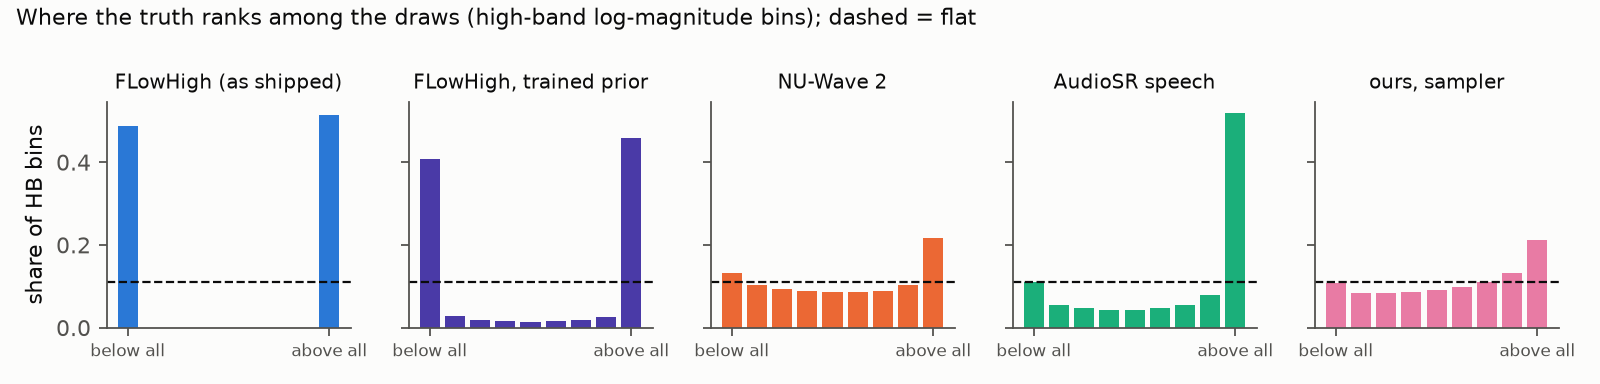
\includegraphics[width=\linewidth]{sota_pit.png}
\caption{Rank of the truth among eight draws, HB log-magnitude bins, \texttt{core}. Dashed: flat. FLowHigh
collapses to a point. AudioSR puts the truth above every draw in 52\% of bins, a level bias. Our sampler's
excess is one-sided (top tail 0.21, bottom 0.11): a residual level bias rather than too narrow an ensemble.}\label{fig:pit}
\end{figure}

\begin{figure}[H]\centering
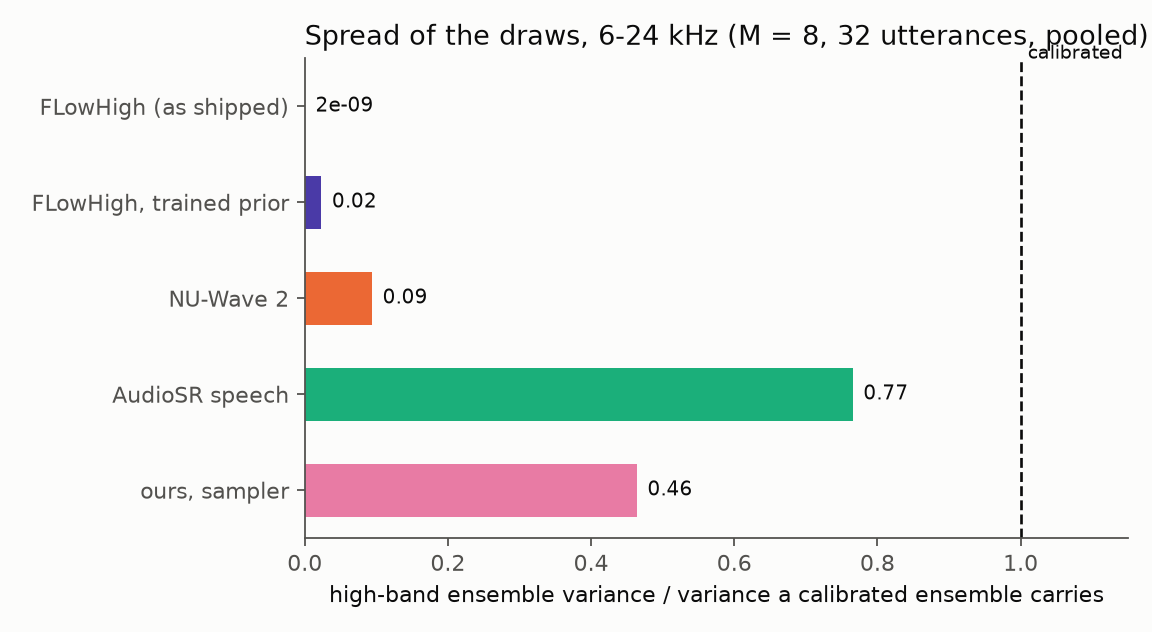
\includegraphics[width=0.7\linewidth]{sota_calibration.png}
\caption{HB spread ratio, \texttt{core}. 1 = calibrated.}\label{fig:spread}
\end{figure}

\subsection{Level against brightness}
\begin{table}[H]\small\centering
\begin{tabular}{lrrr}
\toprule
model & slope (dB/dB) & r & n \\
\midrule
FLowHigh & $-$0.075 & $-$0.16 & 240 \\
AP-BWE & $-$0.119 & $-$0.26 & 240 \\
NU-Wave 2 & $-$0.315 & $-$0.48 & 240 \\
AudioSR (speech) & $-$0.338 & $-$0.47 & 240 \\
det\_paper & $-$0.346 & $-$0.43 & 240 \\
det & $-$0.223 & $-$0.36 & 240 \\
es\_marg & $-$0.239 & $-$0.39 & 240 \\
es\_dec & $-$0.261 & $-$0.41 & 240 \\
es\_erb & $-$0.287 & $-$0.48 & 240 \\
es\_erb, $\lambda{=}0.1$ & $-$0.251 & $-$0.38 & 240 \\
es\_erb, $\lambda{=}0.001$ & $-$0.196 & $-$0.31 & 240 \\
es\_dec\_erb, $\lambda{=}0.1$ & $-$0.235 & $-$0.36 & 240 \\
\bottomrule
\end{tabular}

\caption{Slope of the per-utterance deficit against the truth's HB share, \texttt{wide}. The two models that read
a whole frame or more (FLowHigh, AP-BWE) track the utterance; every objective we trained sits between $-0.20$ and
$-0.35$, whatever its mean level.}\label{tab:slope}
\end{table}

\subsection{Perceptual scores}
\begin{table}[H]\small\centering
\begin{tabular}{lrrrr}
\toprule
condition & ViSQOL audio & NSIM audio & ViSQOL speech & PESQ wb \\
\midrule
FLowHigh & 3.61 & 0.901 & 4.25 & 4.46 \\
FLowHigh, prior restored & 3.62 & 0.902 & 4.25 & 4.47 \\
AP-BWE & 3.48 & 0.881 & 4.05 & 4.36 \\
AP-BWE, own sinc input & 3.49 & 0.885 & 4.12 & 4.36 \\
NU-Wave 2 & 2.57 & 0.771 & 3.07 & 3.95 \\
AudioSR (speech) & 2.41 & 0.780 & 3.73 & 3.89 \\
det\_paper & 1.85 & 0.745 & 3.94 & 4.45 \\
det & 3.13 & 0.853 & 4.12 & 4.35 \\
es\_marg & 2.77 & 0.812 & 3.81 & 4.05 \\
es\_dec & 2.79 & 0.817 & 3.90 & 4.07 \\
es\_erb & 2.82 & 0.821 & 3.96 & 4.09 \\
es\_erb, $\lambda{=}0.1$ & 2.86 & 0.828 & 4.02 & 4.04 \\
es\_erb, $\lambda{=}0.001$ & 2.63 & 0.771 & 3.20 & 3.73 \\
es\_dec\_erb, $\lambda{=}0.1$ & 2.83 & 0.823 & 4.01 & 4.12 \\
\bottomrule
\end{tabular}

\caption{\texttt{wide}, draw 0. ViSQOL audio mode spans 1.57 (empty band) to 4.73 (true band) on this task.
Speech-mode ViSQOL and PESQ stop at 8\,kHz and see only 6--8\,kHz of the missing band.}
\end{table}

\begin{figure}[H]\centering
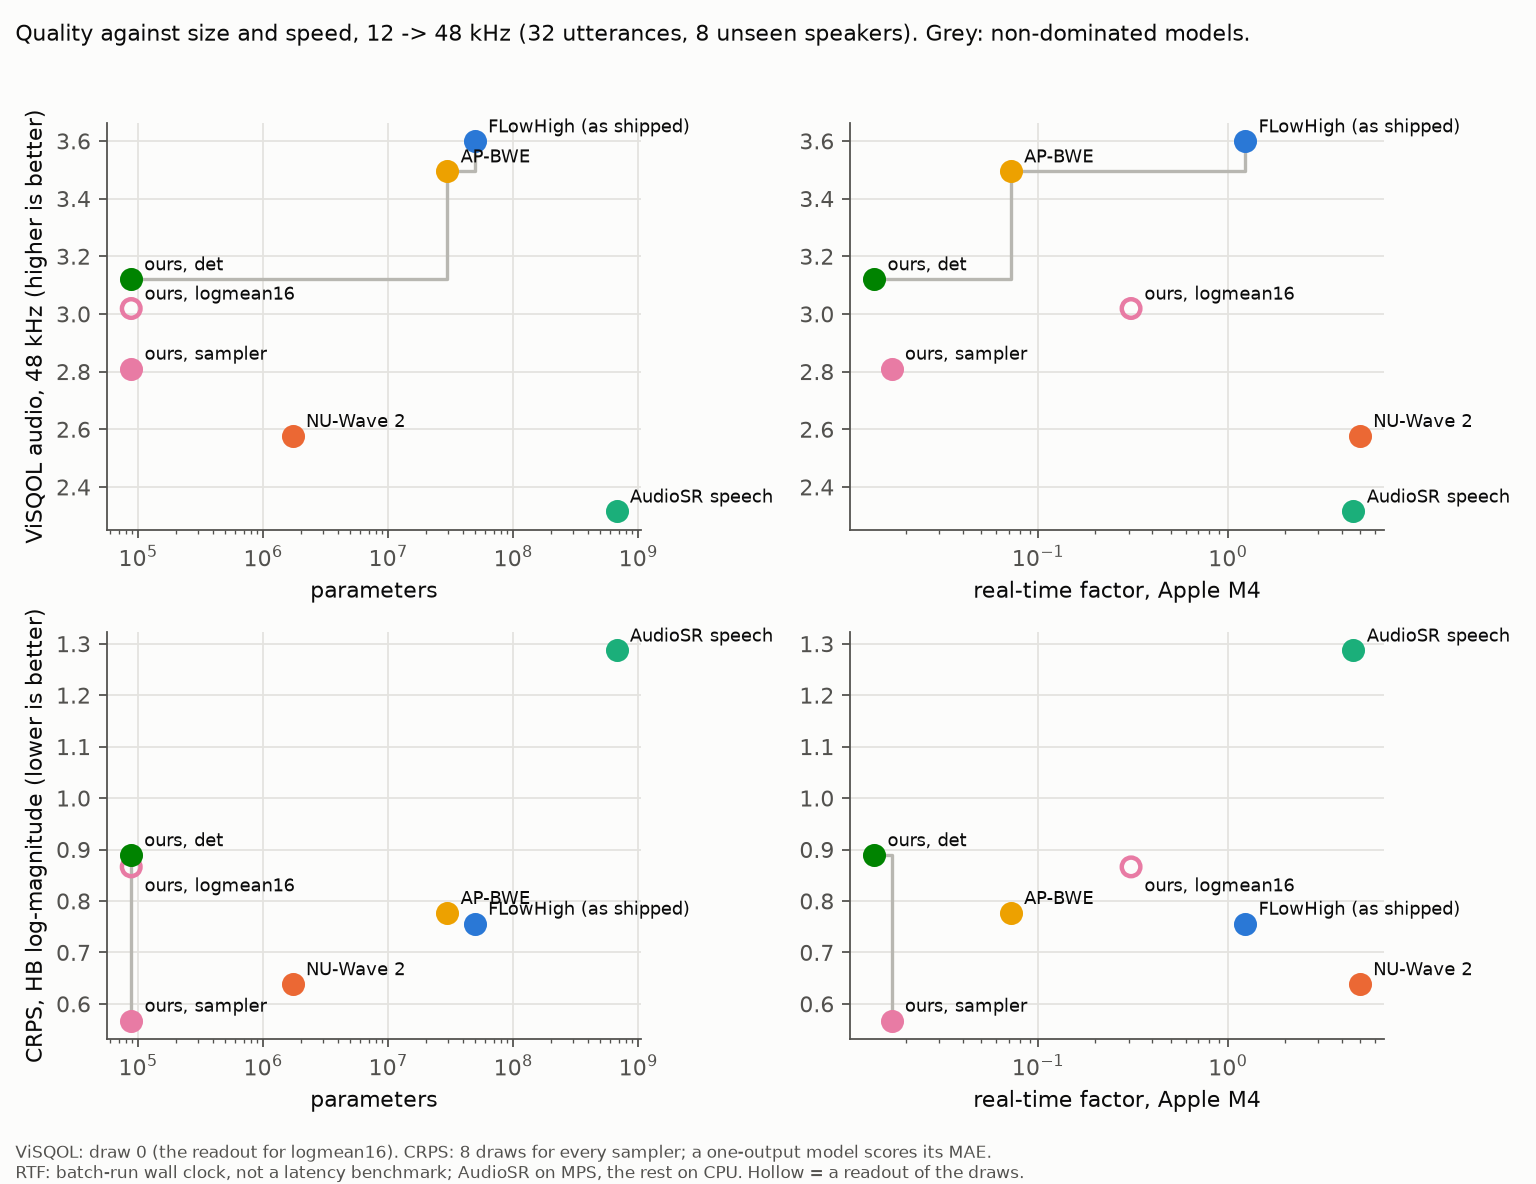
\includegraphics[width=\linewidth]{sota_pareto.png}
\caption{Quality against size and speed, \texttt{core}. This figure uses the all-pairs CRPS and FLowHigh as
shipped; Table~\ref{tab:t2} uses the fair estimator and FLowHigh with its prior restored.}
\end{figure}

\begin{figure}[H]\centering
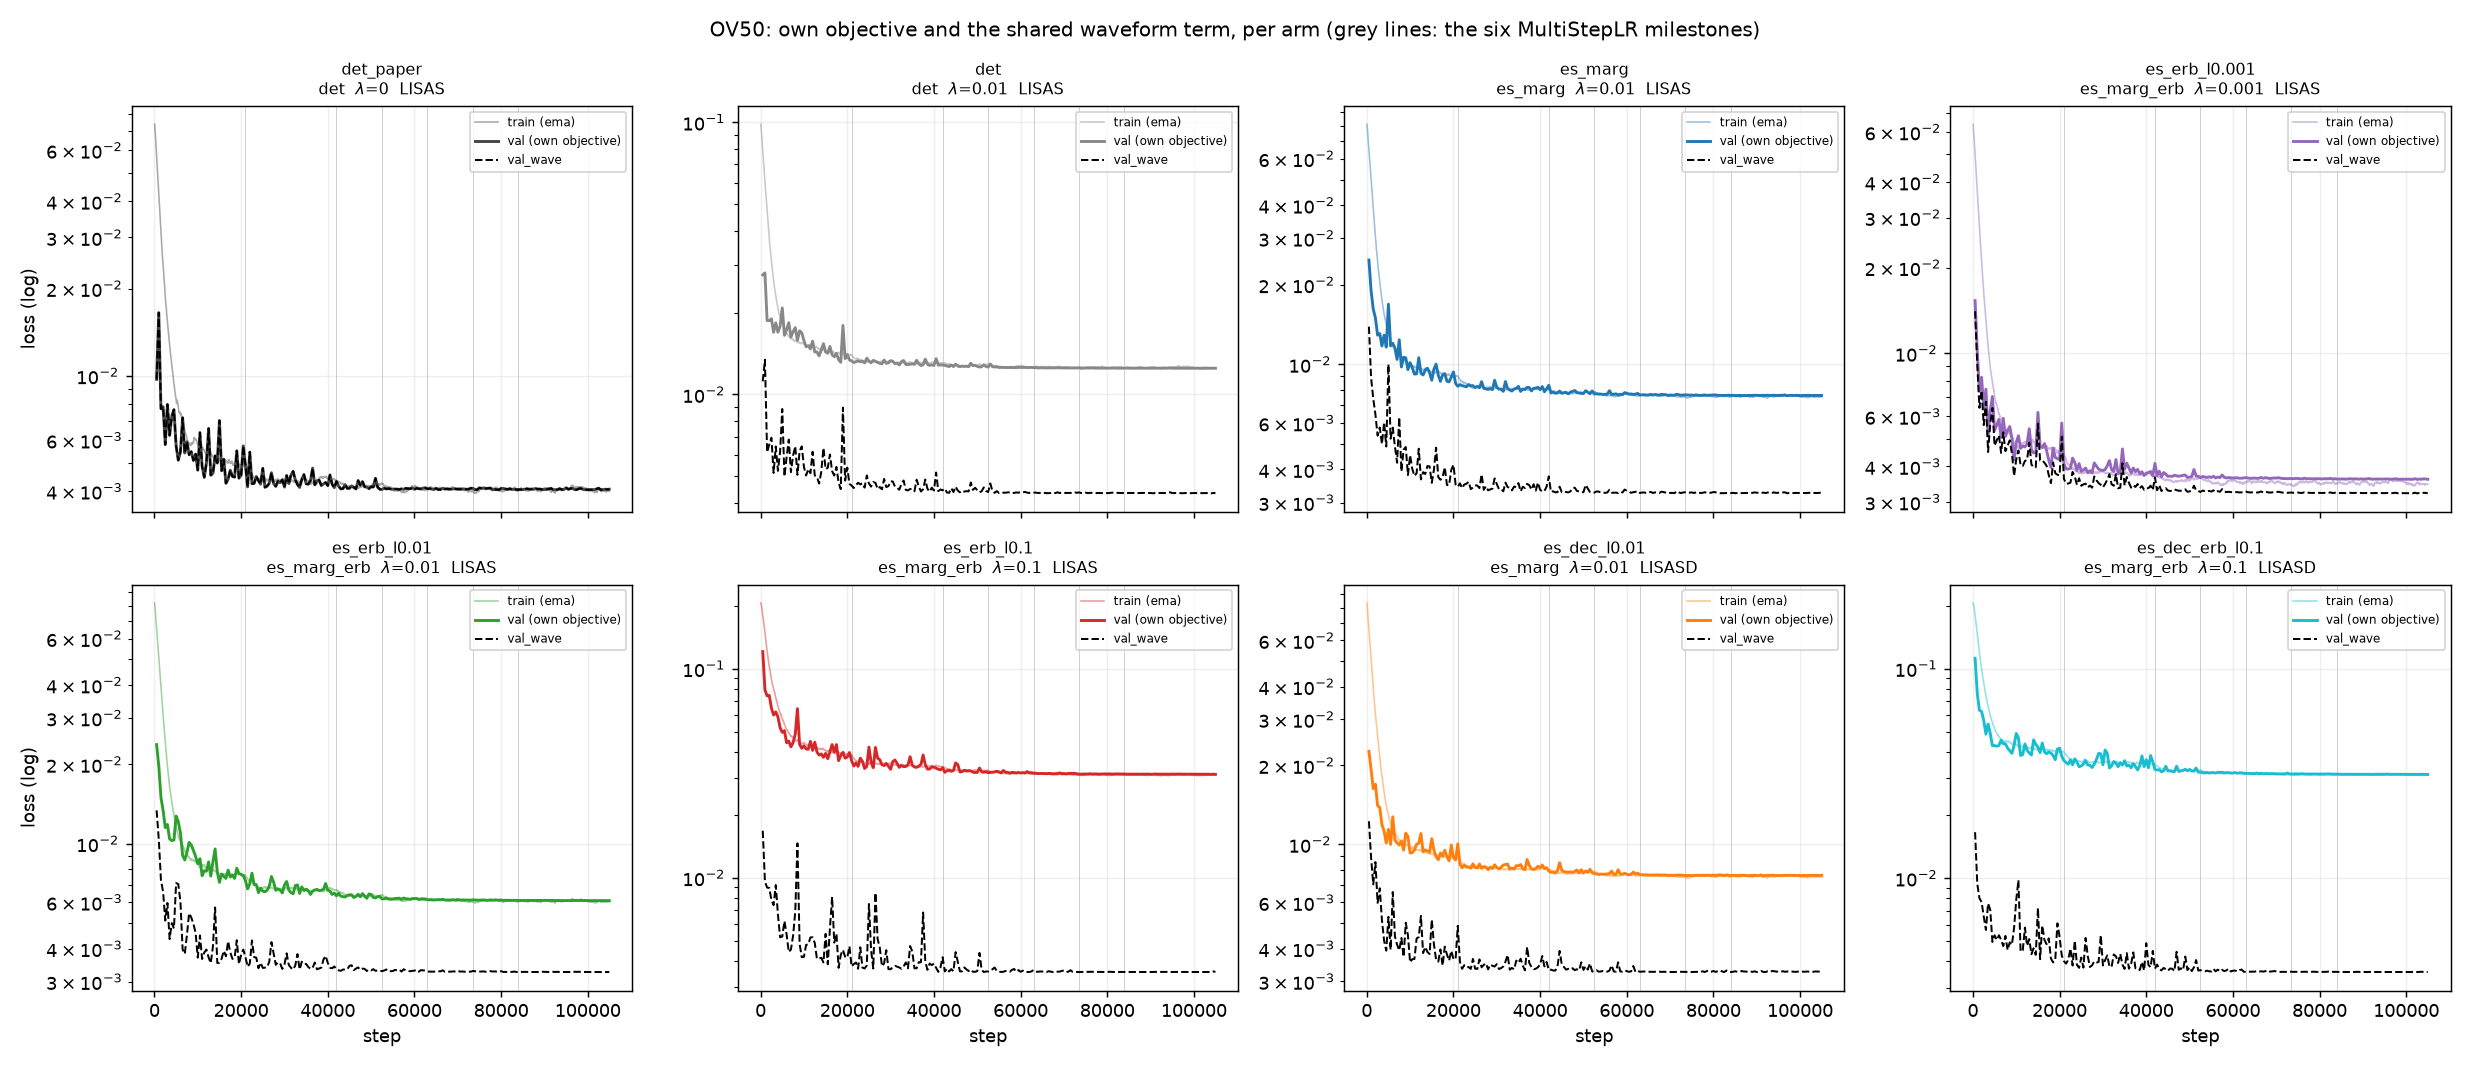
\includegraphics[width=\linewidth]{training_curves.png}
\caption{Training and validation curves of the eight arms (one run each, identical batches).}\label{fig:train}
\end{figure}

%------------------------------------------------------------------------------------------------------------
\section{Limitations}\label{sec:limits}
\begin{itemize}
\item \textbf{No listening test.} ViSQOL and LSD favour FLowHigh and AP-BWE; CRPS favours the samplers. Which
ordering listeners share is not settled here. A proper score ranks predictive distributions, not the
perceptual quality of one draw.
\item \textbf{Small calibration set, one seed.} 32 utterances $\times$ 8 draws; one training seed per arm.
Ranks and bins are correlated within an utterance, so binomial error bars would be too narrow. Utterance-level
bootstrap intervals need the per-utterance score files, which \file{score.py} writes but which are not
included here.
\item \textbf{Scored features.} CRPS is scored per bin on HB log-magnitude. It is proper for each marginal,
not for the joint (\S\ref{sec:es}), and the logarithm weights quiet bins heavily. Sliced CRPS and corr err
cover part of the joint.
\item \textbf{Different spaces.} Spread and gap are measured on the HB waveform; CRPS and PIT on log-magnitude.
\item \textbf{Input-filter mismatch.} Our arms were trained on \texttt{resample\_poly} input and tested on the
Chebyshev input. On p236--p238 this moves the deficit by 0.04--0.07\,dB.
\item \textbf{Training-data overlap.} \texttt{ourtest} is seen by three released models, and AudioSR's data may
include every test speaker (Table~\ref{tab:seen}).
\item \textbf{One test corpus.} VCTK read speech only, 12$\to$48\,kHz only for the calibration results.
\end{itemize}

%------------------------------------------------------------------------------------------------------------
\section{Related work: proper scoring and this argument}\label{sec:related}
\begin{itemize}
\item \textbf{BWE evaluation.} Evaluation sections of 119 BWE and audio super-resolution papers (2017 to
September 2026) were searched. None evaluates with a strictly proper scoring rule or a calibration
diagnostic, and none reports a held-out likelihood, including models trained by likelihood (WaveNet BWE,
WSRGlow, UDM+, CVAE BWE).
\begin{itemize}
\item Diffusion restoration work suggests the spread of several draws as an uncertainty measure
\cite{lemercier2024}.
\item Inference-time search measures spread across AudioSR draws but treats it as noise to select over
\cite{jin2026}.
\item BABE and CQT-Diff add set-level Fr\'echet distances \cite{moliner2024}.
\end{itemize}
\item \textbf{Other fields.} The protocol used here (CRPS, rank histograms, spread-skill) is standard in
stochastic downscaling of weather and climate fields, which is super-resolution by another name
\cite{leinonen2021,harris2022,mardani2025}. A general inverse-problem version was proposed in 2026
\cite{baattrup2026}.
\item \textbf{Earlier statements of the argument.} The steps before it are established:
\begin{itemize}
\item BWE is ill-posed \cite{jax2002,bruna2016};
\item regression returns a muffled mean \cite{zen2009,lemercier2023storm,fu2026};
\item SNR rewards an empty band \cite{su2021,han2022}.
\end{itemize}
Speech synthesis also found that samples beat the mean only when the model is accurate \cite{henter2018}, and
classical BWE biased the band quieter on purpose, because over-estimation is judged more harshly
\cite{nilsson2001}.
\end{itemize}
Our contribution is the measurement applied to released BWE systems, and what it finds there.

%------------------------------------------------------------------------------------------------------------
\section{Reproducing}
\begin{enumerate}
\item \textbf{Environment.} \file{code/README.md} lists the three Python environments. It also gives two CPU
tests (31 and 18 checks), which pass on this snapshot.
\item \textbf{Train.} \file{code/fast/train_arm.py}, one arm per GPU, about 3\,h each.
\item \textbf{Evaluate.} \file{code/sota/run_all.sh}: inputs, released models, our arms, the scorer, the
mean-of-$M$ table and the figures.
\item \textbf{Tables.} \file{results/make_tables.py} rebuilds every table in this appendix and checks each
number printed in the paper against \file{results/results.json} (\file{results/number_check.md}: all 68
match).
\end{enumerate}

\begin{thebibliography}{99}\small
\bibitem{allen2023} S.~Allen, D.~Ginsbourger, J.~Ziegel. Evaluating forecasts for high-impact events using transformed kernel scores. \emph{SIAM/ASA J.\ Uncertainty Quantification} 11, 2023.
\bibitem{baattrup2026} M.~H.~Baattrup et al. Pointwise metrics mislead: an evaluation protocol for multimodal inverse problems. arXiv:2605.22891, 2026.
\bibitem{bruna2016} J.~Bruna, P.~Sprechmann, Y.~LeCun. Super-resolution with deep convolutional sufficient statistics. ICLR 2016.
\bibitem{ferro2008} C.~A.~T.~Ferro, D.~S.~Richardson, A.~P.~Weigel. On the effect of ensemble size on the discrete and continuous ranked probability scores. \emph{Meteorological Applications} 15, 2008.
\bibitem{freirich2021} D.~Freirich, T.~Michaeli, R.~Meir. A theory of the distortion-perception tradeoff in Wasserstein space. NeurIPS 2021.
\bibitem{fu2026} S.-W.~Fu et al. Rethinking training targets, architectures and data quality for universal speech enhancement. arXiv:2603.02641, 2026.
\bibitem{gneiting2007} T.~Gneiting, A.~E.~Raftery. Strictly proper scoring rules, prediction, and estimation. \emph{JASA} 102, 2007.
\bibitem{gritsenko2020} A.~Gritsenko et al. A spectral energy distance for parallel speech synthesis. NeurIPS 2020.
\bibitem{han2022} S.~Han, J.~Lee. NU-Wave 2: A general neural audio upsampling model for various sampling rates. Interspeech 2022.
\bibitem{harris2022} L.~Harris et al. A generative deep learning approach to stochastic downscaling of precipitation forecasts. \emph{JAMES} 14, 2022.
\bibitem{henter2018} G.~E.~Henter, S.~King, T.~Merritt, G.~Degottex. Analysing shortcomings of statistical parametric speech synthesis. arXiv:1807.10941, 2018.
\bibitem{jax2002} P.~Jax, P.~Vary. An upper bound on the quality of artificial bandwidth extension of narrowband speech signals. ICASSP 2002.
\bibitem{jin2026} Y.~Jin et al. Inference-time scaling for diffusion-based audio super-resolution. AAAI 2026.
\bibitem{leinonen2021} J.~Leinonen, D.~Nerini, A.~Berne. Stochastic super-resolution for downscaling time-evolving atmospheric fields with a generative adversarial network. \emph{IEEE TGRS} 59, 2021.
\bibitem{lemercier2023storm} J.-M.~Lemercier, J.~Richter, S.~Welker, T.~Gerkmann. StoRM: A diffusion-based stochastic regeneration model for speech enhancement and dereverberation. \emph{IEEE/ACM TASLP} 31, 2023.
\bibitem{lemercier2024} J.-M.~Lemercier et al. Diffusion models for audio restoration: a review. \emph{IEEE Signal Processing Magazine} 41(6), 2024.
\bibitem{liu2022} X.~Liu, C.~Gong, Q.~Liu. Flow straight and fast: learning to generate and transfer data with rectified flow. arXiv:2209.03003, 2022.
\bibitem{mardani2025} M.~Mardani et al. Residual corrective diffusion modeling for km-scale atmospheric downscaling. \emph{Communications Earth \& Environment} 6, 2025.
\bibitem{moliner2024} E.~Moliner, F.~Elvander, V.~V\"alim\"aki. Blind audio bandwidth extension: a diffusion-based zero-shot approach. \emph{IEEE/ACM TASLP} 32, 2024.
\bibitem{nilsson2001} M.~Nilsson, W.~B.~Kleijn. Avoiding over-estimation in bandwidth extension of telephony speech. ICASSP 2001.
\bibitem{ohayon2023} G.~Ohayon, T.~Adrai, M.~Elad, T.~Michaeli. Reasons for the superiority of stochastic estimators over deterministic ones: robustness, consistency and perceptual quality. ICML 2023.
\bibitem{su2021} J.~Su, Y.~Wang, A.~Finkelstein, Z.~Jin. Bandwidth extension is all you need. ICASSP 2021.
\bibitem{zen2009} H.~Zen, K.~Tokuda, A.~W.~Black. Statistical parametric speech synthesis. \emph{Speech Communication} 51, 2009.
\end{thebibliography}

\end{document}
